% !TEX encoding = UTF-8 Unicode
\documentclass{article}

\usepackage{polski}
\usepackage[utf8]{inputenc}
\usepackage{subfig}
\usepackage{graphicx}
\usepackage{hyperref}
\usepackage{newfloat}
\usepackage[a4paper, left=1.5cm, right=1.5cm, top=3.0cm, bottom=2.0cm, headsep=2.5cm]{geometry}

\linespread{1.3}
\DeclareFloatingEnvironment[fileext=lop]{Tabela}	
\begin{document}

	\begin{titlepage}
		\centering
		{\scshape\LARGE Politechnika Wrocławska \par}
		{\scshape\Large Katedra Systemów i Sieci Komputerowych \par}
		
		\vspace{1cm}
		{\scshape\Large Technologie Sieciowe 2\par}
		\vspace{5cm}
		{\huge\bfseries Projekt przedmiotowy\par}
		\vspace{5cm}
		{\Large\itshape Magdalena Biernat, 225934\par}
		{\Large\itshape Michał Duński, 226081\par}
		\vfill
		Opiekun\par
		dr inż. Michał Kucharzak 
		
		\vfill
		{\large \today\par}
	\end{titlepage}
	\newpage
	\section{Wstęp}
	 Zadaniem tego projektu jest zaprojektowanie sieci komputerowej dla firmy RoboNet - przedsiębiorstwa zajmującego się produkcją oprogramowania dla specjalistycznych urządzeń ‒ robotów. Firma zatrudnia ok. 180 osób podzielonych na 3 grupy robocze, które zajmują 2 budynki. Budynek A posiada 3 kondygnacje, Budynek B posiada 1 kondygnację. Laboratorium znajduje się na parterze w budynku A. Sieć laboratoryjna nie ma dostępu do internetu. Do sieci laboratoryjnej mają dostęp wyłącznie Programiści i Testerzy. Serwery plików, www i pocztowy znajdują się w Budynku A i mieszczą się na dwóch kondygnacjach. Jeden serwer jest umieszczony w Budynku B.\newline
	 \noindent
	 \newline
Planujemy zastosować odpowiednie programy antywirusowe dla bezpieczeństwa oprogramowania oraz aby ograniczyć dostęp do sieci.
\newline
\noindent
\newline
	Projektowana sieć powinna cechować się jakością, niezawodnością oraz skalowalnością w przypadku potrzeby zwiększenia ilości pracowników w firmie. Ważnym czynnikiem jest również estetyczna jakość wykonania instalacji.
\newpage
\section{Inwentaryzacja zasobów: sprzętu, aplikacji, zasobów ludzkich}
Siedziba firmy mieści się w dwóch budynkach o oznaczeniach A i B. Budynek A jest trzypiętrowy, a budynek B ma tylko parter. 
\subsection{Wykaz pomieszczeń w budynkach}
\begin{enumerate}
	\item Budynek A
	\begin{itemize}
		\item Parter: administratorzy, serwerownia 1, laboratorium, recepcja
		\item Piętro 1: programiści i testerzy, serwerownia pocztowa, serwerownia www, toaleta
		\item Piętro 2: zarząd i kadry, programiści i testerzy, toaleta
	\end{itemize}
	\item Budynek B
		\begin{itemize}
		\item Parter: zarząd i kadry, programiści i testerzy, serwerownia 2, dwie toalety, recepcja
	\end{itemize}
\end{enumerate}
\subsection{Sprzęt}
Firma na wyposażeniu posiada:
\begin{itemize}
	\item 16 robotów
	\item 7 drukarek
	\item 24 kamery IP
\end{itemize}
\begin{Tabela}[!ht]
	\centering
\begin{tabular}{|c|c|c|c|c|}\hline
	\centering
	& Budynek A & Budynek A & Budynek A & 	Budynek B 	\\
	\centering
 & parter & piętro I & pietro II & parter \\
 \hline
drukarki & 1 & 2 & 2 & 2\\
\hline
roboty (urządzenia) & 16 & - & - & - \\
\hline
kamery IP & 8 & 4 & 4 & 8 \\
\hline
\end{tabular}
\caption{Rozkład urządzeń}
\end{Tabela}
\newpage
\section{Analiza potrzeb użytkowników – wymagania zamawiającego}
\subsection{Dostęp do Internetu}
Na podstawie bieżących potrzeb firmy RoboNet(tabela niżej), przy uwzględnieniu ewentualnego rozrostu przedsiębiorstwa oraz obecnych na rynku ofert najlepszym rozwiązaniem w kwestii dostępu do Internetu jest łącze symetryczne 100Mb/100Mb.\newline
W tabeli sumowane są wartości przepływów z i do Internetu dla każdego użytkownika. Wartości są w kb/s.
\newline
\begin{Tabela}[!ht]
	\centering
\begin{tabular}{|c|c|c|} \hline
	& down & up \\
	\hline
	serwer www & 7 680 & 16 320\\
	serwer pocztowy & 10 680 & 4 920\\
	wideorozmowy & 7 040 & 7 040 \\
	komunikator & 9 600 & 9 600 \\
	praca w chmurze & 6 664 & 10 472 \\
	przeglądarka & 24 920 & 5 020 \\
	\hline
	\hline
	SUMA & 66 584 & 53 372\\
	\hline
\end{tabular}
\caption{Wartość przepływów}
\end{Tabela}

\subsection{Sieć lokalna}
W celu zapewnienia wystarczającej przepustowości w sieci lokalnej wykorzystane będzie okablowanie w technologii 100Base-TXFast Ethernet(okablowanie poziome) oraz 1000Base-T Gigabit Ethernet(okablowanie pionowe).  Wymagana przepustowość sieci lokalnej została podana w tabeli poniżej. Wartości zostały sumowane dla przepływów lokalnych dla każdego użytkownika. Wartości są w kb/s.

\begin{Tabela}[!ht]
	\centering
\begin{tabular}{|c|c|c|c|c|c|c|c} \hline
	& Download lokalny, kb/s \\
	\hline
	Użytkownik/aplikacja & Plików 1 & 9Plików 2&WWW&Pocztowy&Drukarka&Liczba&SUMA\\
	\hline
	1. Zarząd i kadry  & 0 & 600&230&330&10&28&32 760\\
	2. Programiści i Testerzy & 0 & 700&190&380&10&148&189 440\\
	3. Administratorzy & 8 000 & 800&210&380&10&4&37 600\\
	4. Kamery & 100 & 0&0&0&0&24&2 400\\
	\hline
	\hline
	&&&&&&SUMA &262 200 \\
	\hline
\end{tabular}
\caption{Download lokalny}
\end{Tabela}
\begin{Tabela}[!ht]
	\centering
	\begin{tabular}{|c|c|c|c|c|c|c|c} \hline
		& Download lokalny, kb/s \\
		\hline
		Użytkownik/aplikacja & Plików 1 & 9Plików 2&WWW&Pocztowy&Drukarka&Liczba&SUMA\\
		\hline
		1. Zarząd i kadry  & 0 & 550 & 45 & 440 & 180 & 28 & 34 020\\
		2. Programiści i Testerzy & 0 & 550 & 30 & 430 & 170 & 148 & 174 640\\
		3. Administratorzy & 600 & 300 & 60 & 390 & 175 & 4 &6 100\\
		4. Kamery & 2 800 & 0 & 0 & 0 & 0 & 24 & 67 200\\
		\hline
		\hline
		&&&&&&SUMA &262 200 \\
		\hline
	\end{tabular}
	\caption{Upload lokalny}
\end{Tabela}

\begin{Tabela}[!ht]
	\centering
	\begin{tabular}{|c|c|c|c|c|c|c} \hline
		& Download lokalny, kb/s \\
		\hline
		Użytkownik/aplikacje & Przeglądarka& Chmura & Komunikator & Wideorozmowy & Liczba &SUMA\\
		\hline
		1. Zarząd i kadry  & 80 & 23 & 15 & 40 & 28 & 4 424\\
		2. Programiści i Testerzy & 110 & 30 & 15 & 40 & 148 & 28 860\\
		3. Administratorzy & 100 & 20 & 20 & 0 & 4 & 560\\
		4. Sieć gości & 20 & 5 & 5 & 0 & 300 & 9 000\\
		\hline
		\hline
		&&&&Download, kb/s && \\
		\hline
		&&& WWW & 80 & 96 & 7 680\\
		&&& Pocztowy & 890 & 12 & 10 680\\
		&&&&&&61 204\\
		\hline
	\end{tabular}
	\caption{Download Internet}
\end{Tabela}
\begin{Tabela}[!ht]
	\centering
	\begin{tabular}{|c|c|c|c|c|c|c} \hline
		& Download lokalny, kb/s \\
		\hline
		Użytkownik/aplikacje & Przeglądarka& Chmura & Komunikator & Wideorozmowy & Liczba &SUMA\\
		\hline
		1. Zarząd i kadry  & 15 & 36 & 15 & 40 & 28 & 2 968\\
		2. Programiści i Testerzy & 10 & 53 & 15 & 40 & 148 & 17 464\\
		3. Administratorzy & 20 & 30 & 30 & 0 & 4 & 320\\
		4. Sieć gości & 20 & 5 & 5 & 0 & 300 & 9 000\\
		\hline
		\hline
		&&&&Download, kb/s && \\
		\hline
		&&& WWW & 170 & 96 & 16 320\\
		&&& Pocztowy &410 & 12 & 4 920\\
		&&&&&&50 992\\
		\hline
	\end{tabular}
	\caption{Upload Internet}
\end{Tabela}
\newpage
\section{Założenia projektowe}
Projekt zakłada stworzenie sieci dla przedsiębiorstwa zajmującego się produkcją oprogramowania dla specjalistycznych urządzeń ‒ robotów, których zastosowanie jest ściśle tajne. Przedsiębiorstwo posiada dwa budynki. W jednym pracuje 100 użytkowników (komputerów, 5 drukarek, 16 kamer IP, 16 robotów i 3 serwery). W drugim pracuje 80 użytkowników (komputerów, 2 drukarki, 8 kamer IP i 1 serwer. W każdym budynku projekt zakłada sieć WiFi dla 150 gości. Budynek A ma trzy kondygnacje, budynek B posiada tylko parter. Przed stworzeniem sieci komputerowej zostanie wykonane (we wcześniejszym terminie i dla odpowiednich pomieszczeń) dostosowanie instalacji elektrycznej.
W obu budynkach będą znajdować się przełączniki warstwy trzeciej.
Dla połączenia z Internetem zostanie zamontowany router chroniony firewallem.
Z sieci gości możliwy jest wyłącznie dostęp do Internetu.
Wszyscy pracownicy mają dostęp do wszystkich drukarek i pozostałych serwerów. Z Internetu możliwy jest dostęp wyłącznie do Serwera WWW i Serwera Pocztowego.
Okablowanie poziome w technologii 100Base-TXFast, okablowanie pionowe w technologii 1000Base-T Gigabit Ethernet oraz połączenie światłowodowe między budynkami. Dla zachowania odpowiedniej estetyki kable zostaną schowane w podłodze lub podwieszanym suficie.
Zastosowanie odpowiednich programów antywirusowych dla bezpieczeństwa oprogramowania oraz ograniczony dostęp do sieci.

\newpage
\section{Projekt sieci}
\subsection{Projekt logiczny wraz z opisem koncepcji rozwiązania i uzasadnieniem}
\begin{figure}[!ht]	
	\centering
	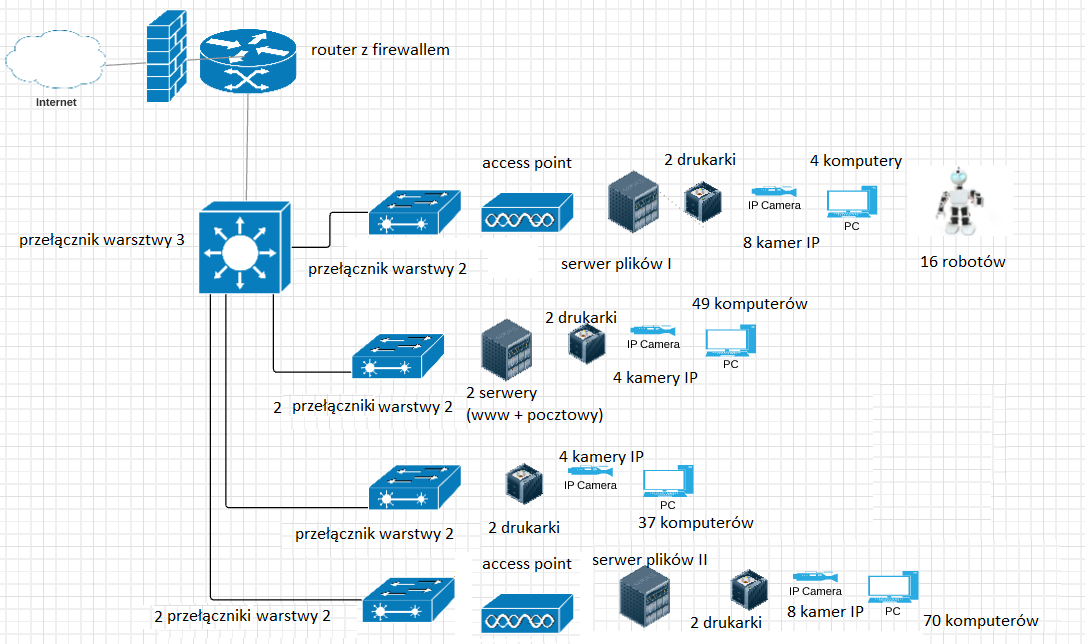
\includegraphics[height=10cm]{projekt_logiczny2.png}
	\caption{Projekt logiczny sieci}
	\label{fig:obrazek 1}
\end{figure}
Dostęp do internetu jest przez router z firewallem. Przełącznik warstwy 3 łączy przełączniki warstwy 2. Każde piętro ma przełącznik lub dwa (zależy od liczby potrzebnych wejść).

\subsection{Wybór urządzeń}
\begin{enumerate}
	\item Przełącznik warstwy 3\newline
	\begin{figure}[!ht]	
		\centering
		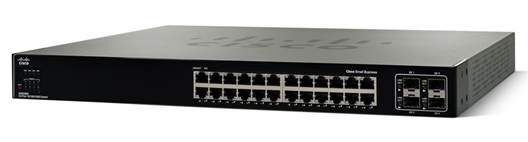
\includegraphics[height=3cm]{1.jpg}
		\caption{przełącznik warstwy 3}
		\label{fig:obrazek 2}
	\end{figure}
	\href{https://www.cisco.com/c/en/us/products/collateral/switches/sge2000-24-port-gigabit-switch/data\_sheet\_c78-502447.html}{Cisco SGE2000}
	\begin{itemize}
		\item 24 porty RJ-45 10BASE-T/100BASE-TX/1000BASE-T
		\item Port konsolowy
		\item Port RPS do podłączenia zapasowego źródła zasilania
	\end{itemize}
	
		\item Przełącznik warstwy 2 - 48 portów
		\begin{figure}[!ht]	
		\centering
		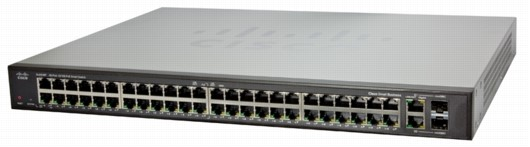
\includegraphics[height=3cm]{2.jpg}
		\caption{przełącznik warstwy 2}
		\label{fig:obrazek 3}
	\end{figure}
	\href{https://www.cisco.com/c/en/us/products/collateral/switches/slm248p-48-port-10-100-2-port-gigabit-smart-switch-sfps-poe/data_sheet_c78-501235.html}{Cisco SLM248P}
	\begin{itemize}
		\item 48 portów RJ-45 10BASE-T/100BASE-TX/1000BASE-T
		\item 2 porty SFP combo
		\item Wbudowany interfejs WWW
	\end{itemize}
	\item Router
	\href{ https://www.cisco.com/c/en/us/products/collateral/routers/rv325-dual-gigabit-wan-vpn-router/datasheet-c78-729726.html}{Cisco RV325-K9-G5}
		\begin{figure}[!ht]	
		\centering
		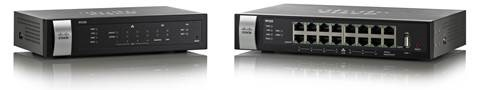
\includegraphics[height=3cm]{3.jpg}
		\caption{router}
		\label{fig:obrazek 4}
	\end{figure}
	\begin{itemize}
		\item 2 porty RJ-45 WAN
		\item Obsługa VPN
	\end{itemize}
	
	\item Serwer
\href{ https://www.cisco.com/c/en/us/products/collateral/servers-unified-computing/ucs-c-series-rack-servers/datasheet-c78-739281.html}{Cisco UCS C220 M5 Rack Server}
		\begin{figure}[!ht]	
		\centering
		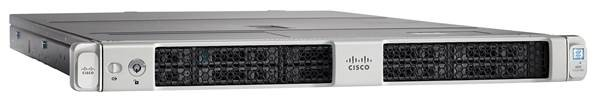
\includegraphics[height=3cm]{4.jpg}
		\caption{serwer}
		\label{fig:obrazek 5}
	\end{figure}
	
	\item Access Point
	\href{ https://www.cisco.com/c/en/us/products/collateral/wireless/aironet-1850-series-access-points/datasheet-c78-734256.html}{Cisco Aironet 1850 Series}
		\begin{figure}[!ht]	
		\centering
		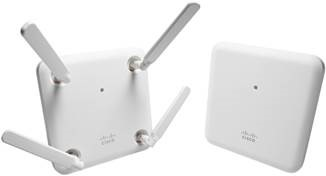
\includegraphics[height=3cm]{5.jpg}
		\caption{przełącznik warstwy3}
		\label{fig:obrazek 6}
	\end{figure}
	\begin{itemize}
		\item Agregacja pakietów A-MPDU (Tx/Rx), A-MSDU (Tx/Rx)
		\item Kanały 20 i 40 MHz
		\item Liczba nienakładających się kanałów
		\begin{itemize}
			\item 2.4GHz
			\begin{itemize}
			\item 802.11b/g - 3
			\item 802.11n - 3
			\end{itemize}
			\item 5GHz
			\begin{itemize}
				\item 802.11a 
			\end{itemize}
		\item 20 MHz - 25
		\begin{itemize}
			\item 802.11n
		\end{itemize}
		\item 20 MHz - 25
		\item 40 MHz - 12
		\begin{itemize}
			\item 802.11ac
		\end{itemize}
		\item 20 MHz - 21
		\item 40 MHz - 12
		\item 80 MHz - 6
		\end{itemize}
	\end{itemize}
\end{enumerate}
\newpage
\subsection{Projekt adresacji IP}

Adresację IP przeprowadziliśmy w standardzie IPv4. Adresem routera podłączonego do Internetu, jest pierwszy dostępny adres prywatny klasy C, czyli 192.168.0.1, który zarazem jest bramą domyślną dla sieci VLAN.
Szczegółowa adresacja znajduje się poniżej:
\begin{Tabela}[!ht]
	\centering
	\begin{tabular}[!ht]{c|c|c|c|c|c}
	budynek &	piętro &	nazwa urządzenie & adres IP &maska&brama domyślna\\
	\hline
	A	& parter &	switch & 192.168.1.2&/26&192.168.1.1\\
	& &access point	& 192.168.1.3&&\\
	& &2 drukarki	& 192.168.1.4-192.168.1.5&&\\
	& & 8 kamer IP &	192.168.1.6-192.168.1.13&&\\
	& & 4 PC	& 192.168.1.14-192.168.1.17&&\\
	& & 16  robotów &	192.168.1.18-192.168.1.33&&\\ \hline
	
	A&I piętro	&2 switche	&192.168.3.2-192.168.3.4&/26&192.168.3.1\\
	&&2 serwery	&192.168.3.5-192.168.3.6&&\\
	&&2 drukarki&	192.168.3.6-192.168.3.7&&\\
	&&4 kamery	&192.168.3.8-192.168.3.11&&\\
	&&49 PC	&192.168.3.12-192.168.3.60&&\\
	\hline
	
	A &II piętro&	2 switche&	192.168.3.66-192.168.3.67&/25&192.168.3.65\\
	&&2 drukarki	&192.168.3.68-192.168.3.69&&\\
	&&4 kamery	&192.168.3.70-192.168.3.73&&\\
	&&37 PC	&192.168.3.74-192.168.3.110&&\\
	\hline
	A & &	WiFi	 &192.168.2.2-192.168.2.254&/25&192.168.2.1\\
	\hline
	\hline
	
	bud B &	parter&2 switche&	192.168.4.2-192.168.4.3&/25&192.168.4.1\\
	&& access point	&192.168.4.4&&\\
	&&2 serwery	&192.168.4.5-192.168.4.6&&\\
	&&2 drukarki&	192.168.4.7-192.168.4.8&&\\
	&&8 kamer	&192.168.4.9-192.168.4.16&&\\
	&&70 PC	&192.168.4.17-192.168.4.86&&\\
	\hline
	&&WiFi &	192.168.5.2-192.168.5.254&/25&192.168.5.1\\
	\hline
	
\end{tabular}
\caption{Adresacja IP}
\end{Tabela}
\newpage
\subsection{Projekt konfiguracji urządzeń}
Poniżej przedstawiony został projekt konfiguracji urządzeń.
\begin{Tabela}[!ht]
	\centering
	\begin{tabular}{c|c|c}
		nazwa urządzenia & urządzenie docelowe &porty\\
		\hline	
		S/A/0/1 &	drukarki&	F0/1-F0/2\\
		&kamery IP	&F0/3-F0/10\\
		&PC	&F0/11-F0/14\\
		&accsess point&	F0/15\\
		\hline
		
		S/A/1/1&	serwery&	F0/1-F0/2\\
		&drukarki&	F0/2-F0/3\\
		&kamery&	F0/4-F0/7\\
		&PC&	F0/8-F0/16\\
		\hline
		
		S/A/1/2	&PC&	F0/1-F0/40\\
		\hline
		
		S/A/2/1&	drukarki&	F0/1-F0/2\\
		&kamery&F0/3-F0/6\\
		\hline
		
		S/A/2/2&	PC	&F0/1-F0/37\\
		\hline
		
		S/B/0/1	&serwery	&F0/1-F0/2\\
		&drukarki&	F0/3-F0/4\\
		&kamery	&F0/5-F0/12\\
		&access point&	F0/13\\
		&PC	&F0/14-43\\
		\hline
		
		S/B/0/2	&PC	&F0/40\\
		\hline
		R/A/0/1&S/A/0/1&F0\\
		&S/A/1/1&F1\\
		&S/A/1/2&F2\\
		&S/A/2/1&F3\\
		&S/A/2/2&F4\\
		&S/B/0/1&F5\\
		&S/B/0/2&F6\\
		\hline
	\end{tabular}
\caption{Konfiguracja urządzeń}
\end{Tabela}
	
\subsection{Projekt podłączenia do Internetu}
Ze względu na obecne zapotrzebowanie firmy jak i przewidywany wzrost jako główne łącze została wybrana usługa „FTTH Optymalny” dostarczana przez firmę REDE.  Poza dostępem do Internetu REDE oferuje również stały adres IP. Firma posiada również ofertę „FTTH Komfortowy” o wyższej przepustowości, co może okazać się przydatne przy dużym rozroście firmy w przyszłości.

Koszty oferty:
\begin{itemize}
	\item Opłata aktywacyjna – 49zł
\item	Konwerter FTTH -> RJ-45 – 150zł
	\item	Stała opłata miesięczna – 59zł
	\item Zewnętrzny adres IP – 15zł miesięcznie
	Parametry łącza:
	\item	Download – 100Mb/s
	\item Upload – 100Mb/s
	\item Czas trwania umowy – 36 miesięcy
\end{itemize}


Jako łącze zapasowe została wybrana oferta firmy Netia „Internet 100”.  Prędkość wysyłania w tej ofercie jest nieco niższa niż wymagana do w pełni bezproblemowego funkcjonowania sieci, ale wystarczająca dla podtrzymania działania najbardziej krytycznych transferów danych. 

Koszty oferty:
\begin{itemize}
\item 	Opłata aktywacyjna - 29zł
\item 	Utrzymanie łącza telefonicznego – 29.24zł miesięcznie
\item 	Stała opłata miesięczna – 49.90zł
\end{itemize}


Parametry łącza:
\begin{itemize}
\item 	Download – 100Mb/s
\item 	Upload – 50Mb/s
\item 	Czas trwania umowy – 24 miesiące
\end{itemize}



\subsection{Analiza bezpieczeństwa i niezawodności sieci}
Niezbędnym elementem w projekcie sieci komputerowej dla danej firmy jest zapewnienie bezpieczeństwa w razie ewentualnych awarii, uszkodzeń lub innych zagrożeń. Opisane zostały tu konkretne zagrożenia oraz mechanizmy, które mają na celu zapewnienie bezpieczeństwa dla systemu informatycznego i sieci.

\subsubsection{Bezpieczeństo fizyczne}
Podstawowym zabezpieczeniem sieci od strony fizycznej jest wykorzystanie w projekcie standardowych mechanizmów
ochronnych:
\begin{itemize}
	\item większość kabli prowadzona jest w specjalnych korytach PCV
	\item urządzenia przechowywane są w przystosowanych do tego celu szafach
\end{itemize}
\subsubsection{Awaria systemów}
Tutaj najważniejsza jest ochrona danych.  Najgorszy scenariusz to utrata wszystkich danych. Dlatego codziennie po zakończonej pracy (w godzinach nocnych) będzie wykonywany backup danych na serwery zewnętrzne. Trzeba będzie również regularnie serwisować sprzęt. Ważnym elementem ochrony serwerów (oraz innych urządzeń) jest odpowiednie dostosowanie pomieszczenia, w którym dane urządzenia będą się znajdować. Obejmuje to między innymi zapewnienie optymalnych warunków dla sprzętu (m.in. poprzez chłodzenie) oraz zabezpieczenie dostępu przed osobami, które nie mają do tego uprawnień.

\subsubsection{Wirusy}
Takie firmy są bardzo narażone na zarażenie pojedynczych komputerów a w konsekwencji całej sieci. Abu tego uniknąć firma powinna korzystać z oprogramowania antywirusowego, które należy regularnie uaktualniać. Dla zwiększenia zapory została użyta również zapora ogniowa w routerze bezpośrednio połączonym z Internetem.

\subsubsection{Brak zasilania}
Jest to poważny problem dużych firm i mocno on wpływa na dostęp do sieci. Najważniejsze w takiej sytuacji jest zapewnienie bezpieczeństwa dla danych. 
Jednym z rozwiązań jest zastosowanie zasilaczy UPS, które pozwolą bezpiecznie wyłączyć serwery.  W ten sposób będzie można zabezpieczyć dane przechowywane przez serwery. Niestety nie wszystkie komputery da się tak zabezpieczyć.

\subsubsection{Włamania oraz ataki na sieć}
Tutaj również najważniejsze są dane przechowywane na serwerach.
Wykorzystana została zapora ogniowa. Jest to pierwszy etap ochrony.

\subsubsection{WiFi}
Należy zapewnić ochronę przed dostępem do sieci osób, które nie mają upoważnienienia.
Najprostszym elementem ochrony sie WiFi jest ustawienie hasła dostępu. Dodatkowo również transmisje będą szyfrowane poprzez WPA2.

\section{Kosztorys}
\begin{Tabela}[!ht]
	\centering
\begin{tabular}{c|c|c}
	nazwa&szt&cena za sztukę\\
	\hline
	Cisco SGE2000&x1&2 700zł\\
	Cisco SLM248P&x6&1 900zł\\
	Cisco RV325-K9-G5& x1& 1 100 zł\\
	Cisco UCS C220 M5& x4& 7 000 zł\\
	Cisco Aironet 1852i& x2& 2 100 zł\\
	\hline
	\hline
	łącznie &&474 000 zł\\
\end{tabular}
\caption{Kosztorys}
\end{Tabela}
\end{document}